\section{Wallet}
Il wallet consente la memorizzazione di credenziali, il credential issuing da parte di un issuer e la verifiable presentation da parte di un verifier.

\subsection{Registrazione al Wallet}
Per la registrazione occorre fornire un indirizzo email e una password.
\begin{center}
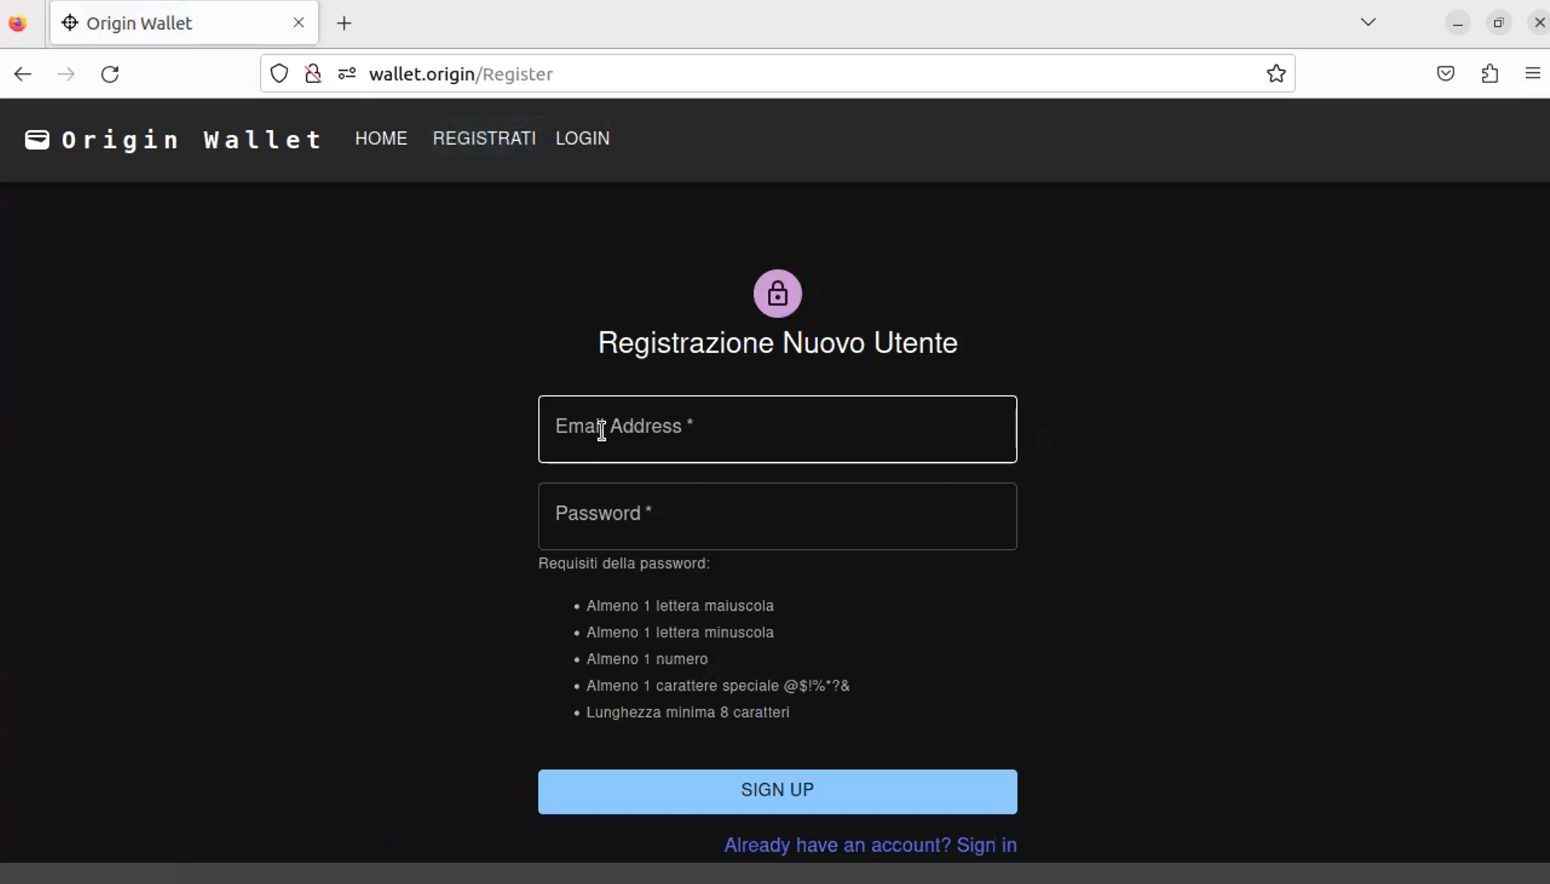
\includegraphics[scale = 0.2]{./res/img/wallet/new/wallet_register.png}
\end{center}

\subsection{Login al Wallet}
Il login si effettua utilizzando email e password utilizzate durante la registrazione.
\begin{center}
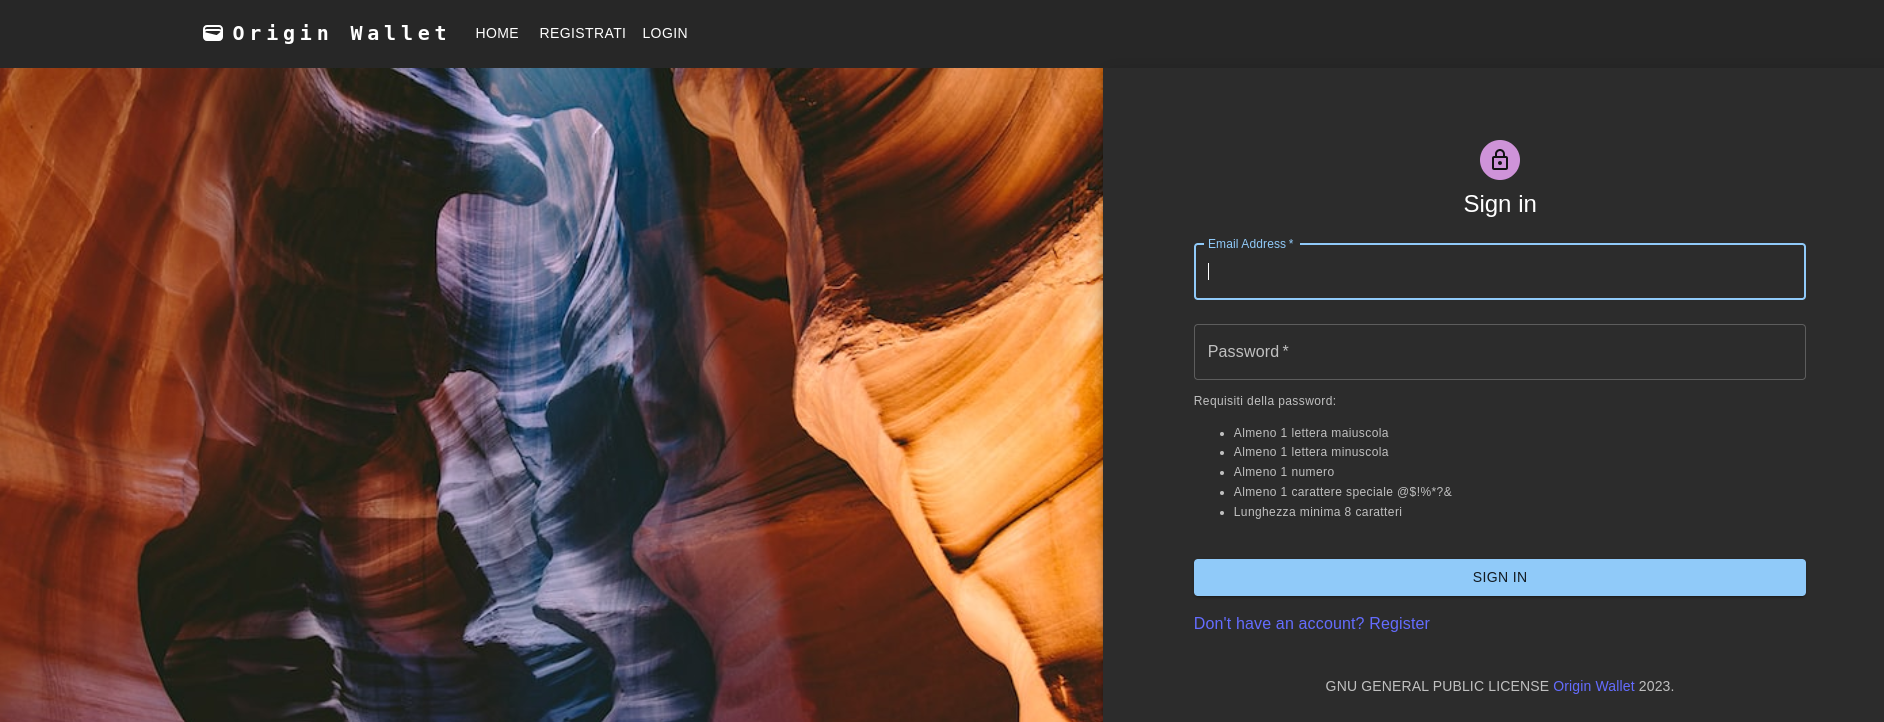
\includegraphics[scale = 0.9]{./res/img/wallet/new/wallet_login.png}
\end{center}

\subsection{Visualizzazione delle proprie credenziali}
Una volta effettuato il login al wallet è possibile vedere la lista delle proprie credenziali. Premendo su \textbf{Dettagli} è possibile vedere tutte le informazioni di una credenziale, e premendo su \textbf{elimina} è possibile eliminare la credenziale.
\begin{center}
    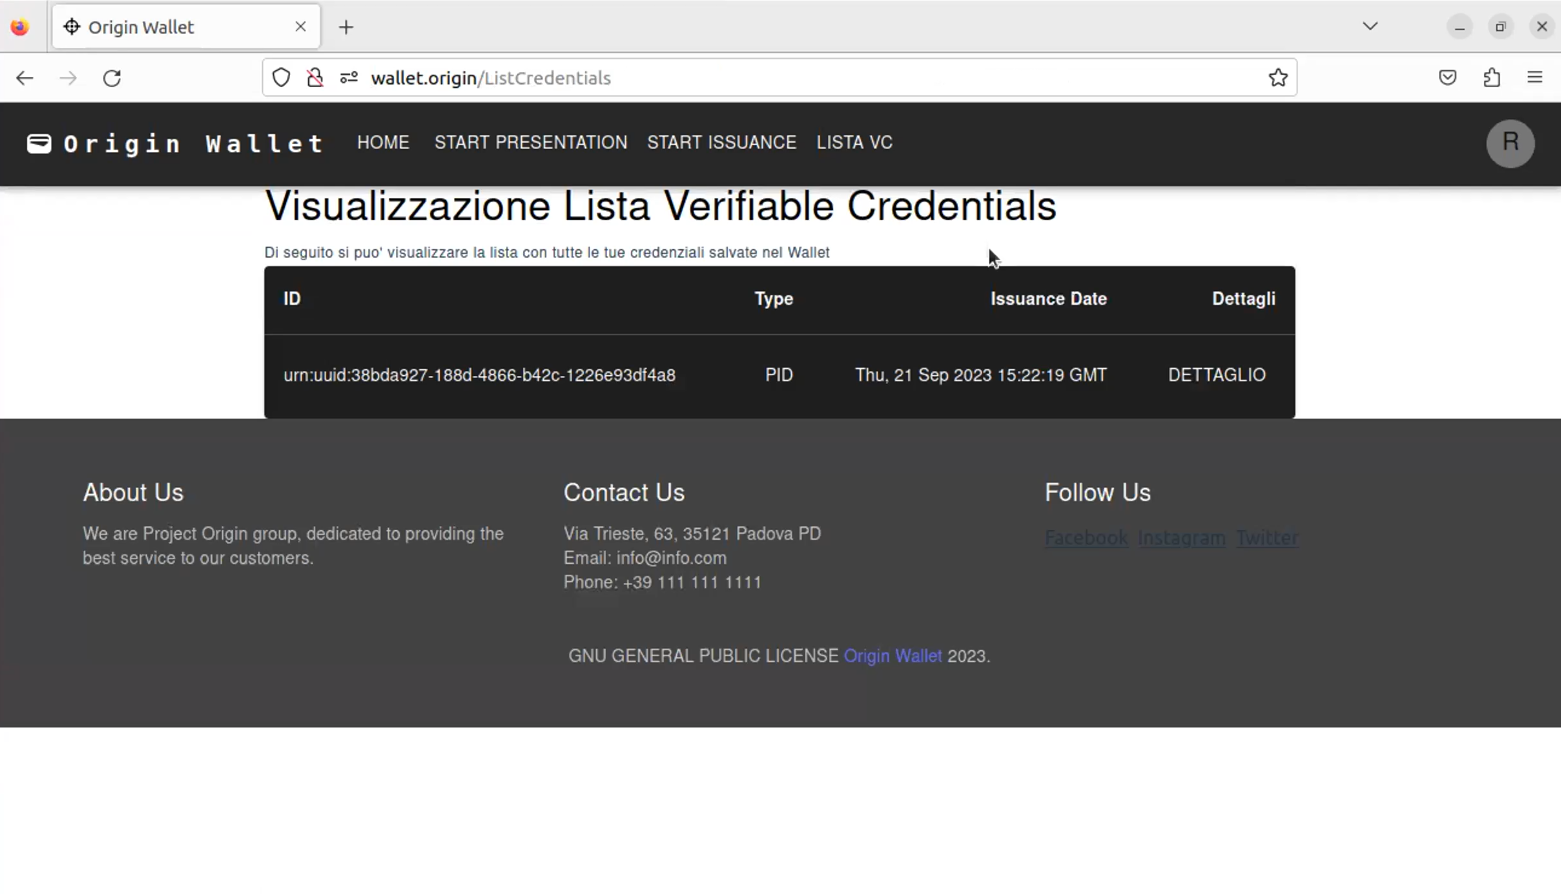
\includegraphics[scale = 0.2]{./res/img/wallet/new/wallet_credential_list.png}
    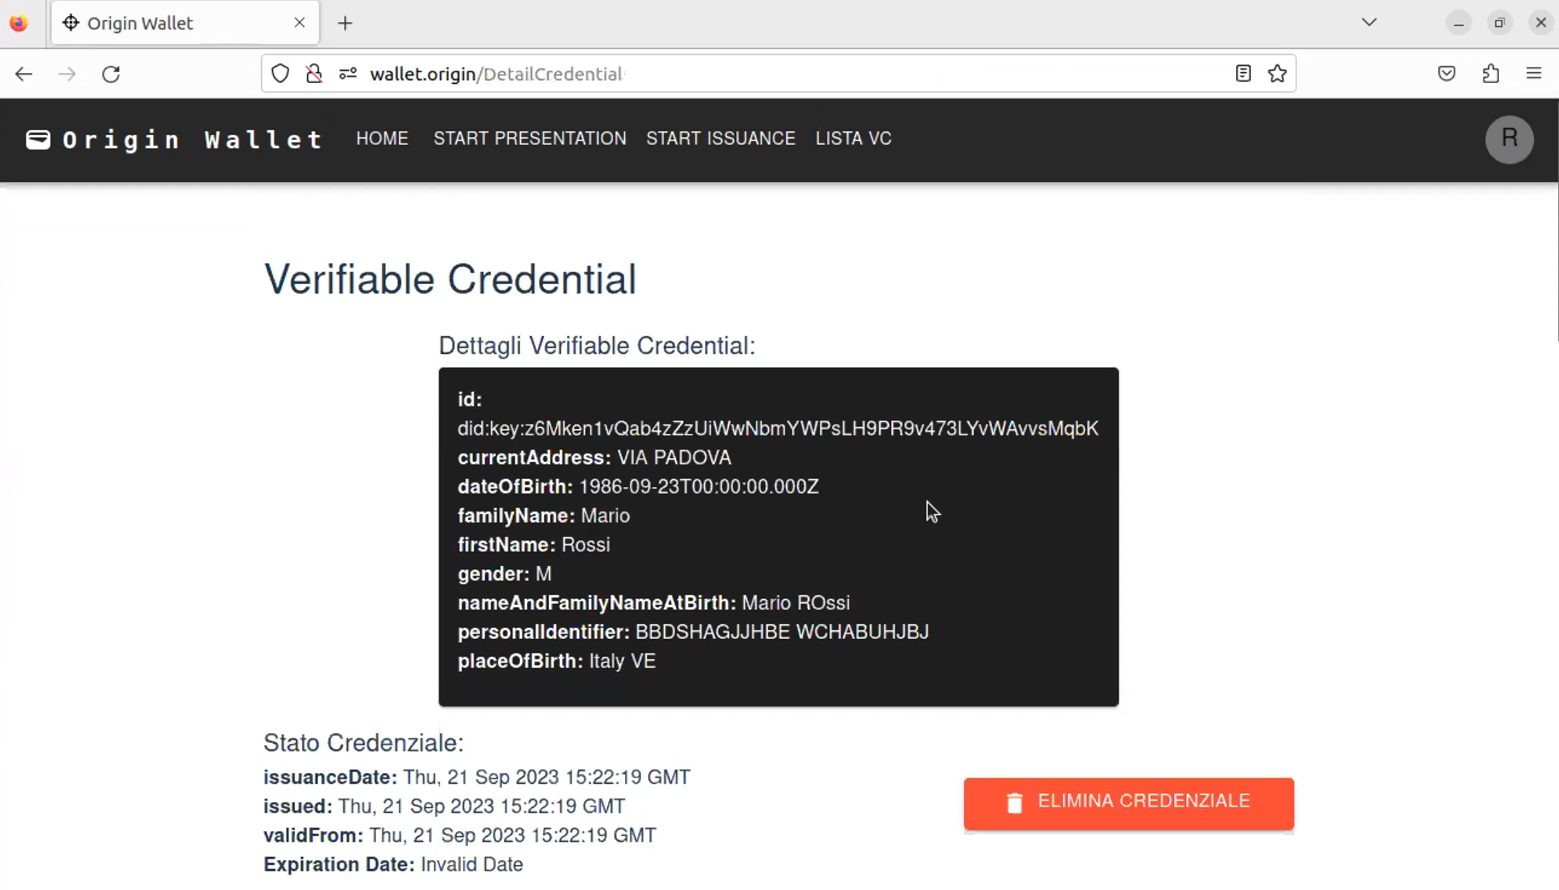
\includegraphics[scale = 0.2]{./res/img/wallet/new/wallet_credential_detail.png}
\end{center}

\subsection{Presentazione di credenziale}
Dopo che si è fatto partire un processo di connessione ad un verifier, per completare la verifiable presentation utilizzando la metodologia cross device, si può utilizzare questa pagina per inserire l'URI openID e continuare la presentazione.\\
Si verrà reindirizzati alla pagina di credential request.
\begin{center}
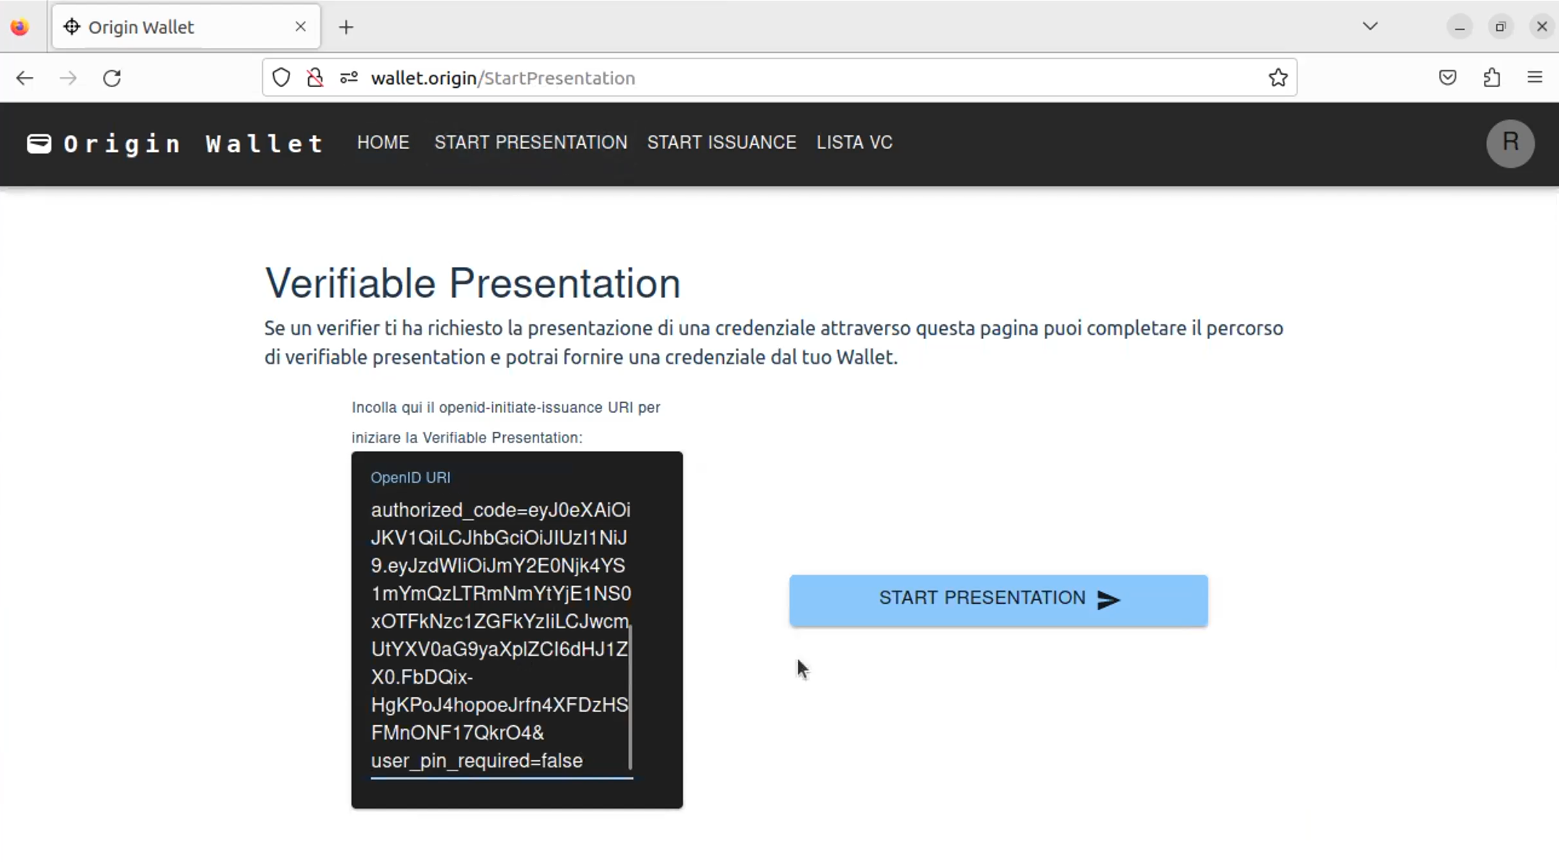
\includegraphics[scale = 0.2]{./res/img/wallet/new/wallet_presentation.png}
\end{center}
\subsection{Pagina Credential Request}
In questa pagina si visualizzano le credenziali presentabili con una verifiable presentation e si selezionano le credenziali che si intende presentare. Premendo il pulsante \textbf{Present} si completerà il processo di presentazione e si verrà reindirizzati al verifier.
\begin{center}
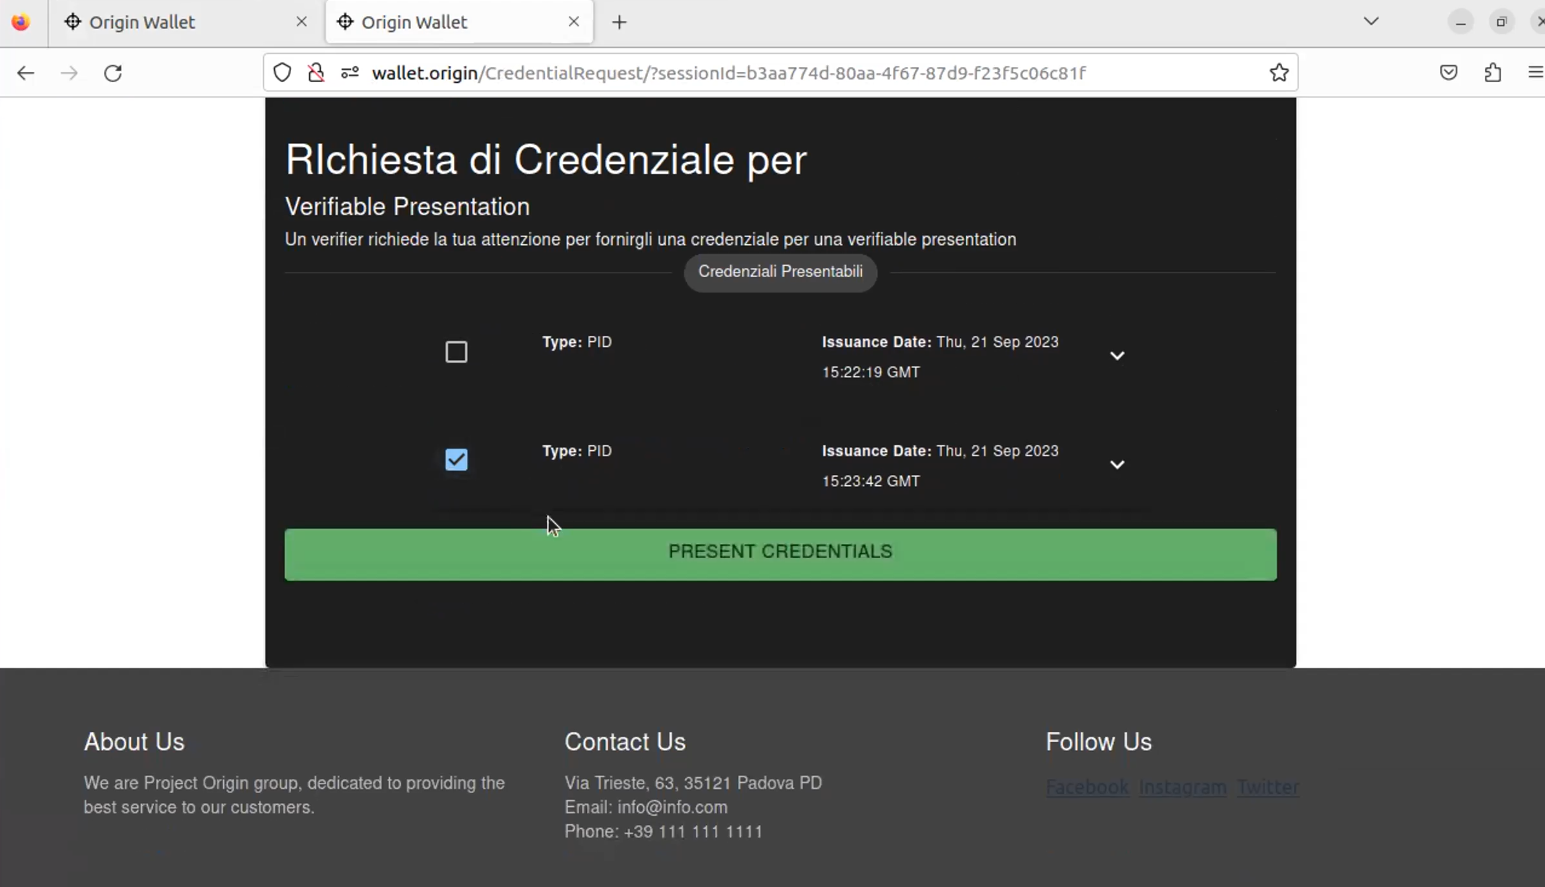
\includegraphics[scale = 0.2]{./res/img/wallet/new/wallet_present.png}
\end{center}